% !TEX root = paper.tex

\section {Results}
\label{sec:results}
\subsection{Flow $p_{\mathrm{T}}$ and multiplicity dependence}

\begin{figure}[h!]
	\centering
	\hspace{-3em}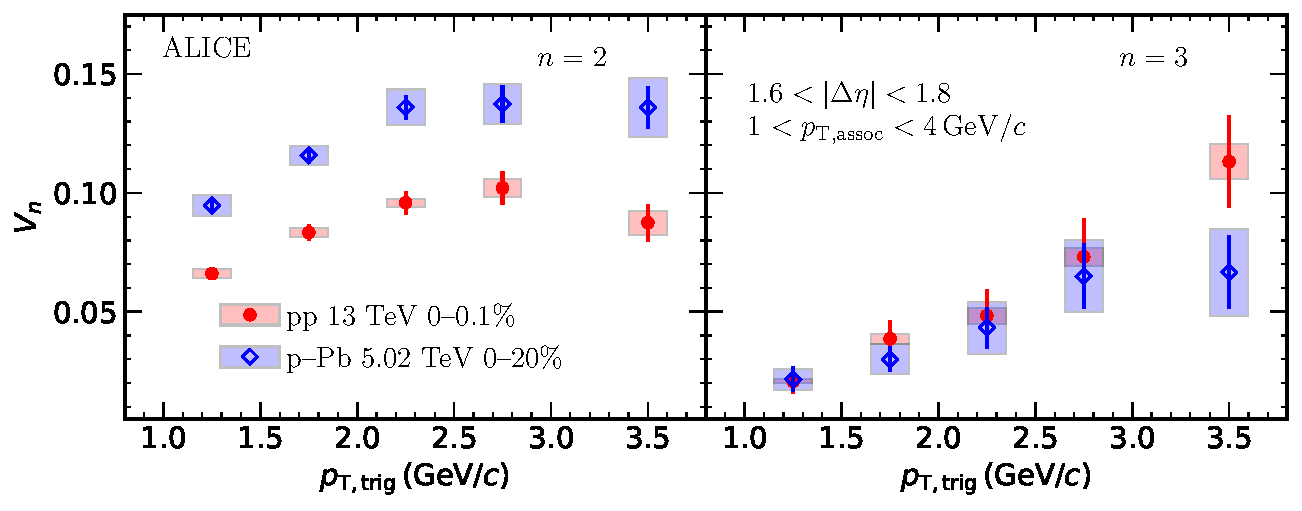
\includegraphics[width=0.9\textwidth]{figures/Fig2_vn_pppPb.pdf} %<--- keep the scale at 0.9 to match with other figures
	\caption{The magnitude of $v_2$ (left) and $v_3$ (right) as a function of $p_\mathrm{T}$ for the high multiplicity percentile of the 0--0.1\% in pp collisions at $\sqrt{s}=13$~TeV and 0--20\% in p--Pb collisions at $\sqrt{s_\mathrm{NN}} = 5.02$~TeV.}
	\label{fig:vn}
\end{figure}

Figure~\ref{fig:vn} shows the extracted values of $v_2$ and $v_3$ as a function of $p_{\mathrm{T,trig}}$ using the low multiplicity template fits. The results were obtained for the high multiplicity percentile of the 0--0.1\% in pp collisions at $\sqrt{s}=13$~TeV and 0--20\% in p--Pb collisions at $\sqrt{s_\mathrm{NN}}=5.02$~TeV. Both results indicate that the magnitudes of $v_n$ increase at higher values of $p_{\mathrm{T,trig}}$. The magnitude of $v_2$ peaks between $2.5<p_{\mathrm{T,trig}}<3.0$ GeV/c, similar to the results from Pb--Pb collisions~\cite{ALICE:2018yph}. A similar trend is seen for $v_3$ within the uncertainties. The magnitudes of $v_2$ in p--Pb collisions are higher than those in pp collisions, which could be attributed to the larger system size and longer-lived medium in p--Pb collisions. However, the magnitudes of $v_3$ are similar in both collisions, indicating that it is less sensitive to the collision systems.
These results are comparable to those obtained by ATLAS in different multiplicity classes, where the same method was used to extract the flow coefficients~\cite{ATLAS:2016yzd}. Even though the $\Delta\eta$ and $p_{\mathrm{T,assoc}}$ ranges are wider in the ATLAS results at $2.0<|\Delta\eta|<5.0$ and $0.5<p_{\mathrm{T,assoc}}<5\,\mathrm{GeV}/c$, respectively, the results are consistent within uncertainties.

\begin{figure}[h!]
	\centering
	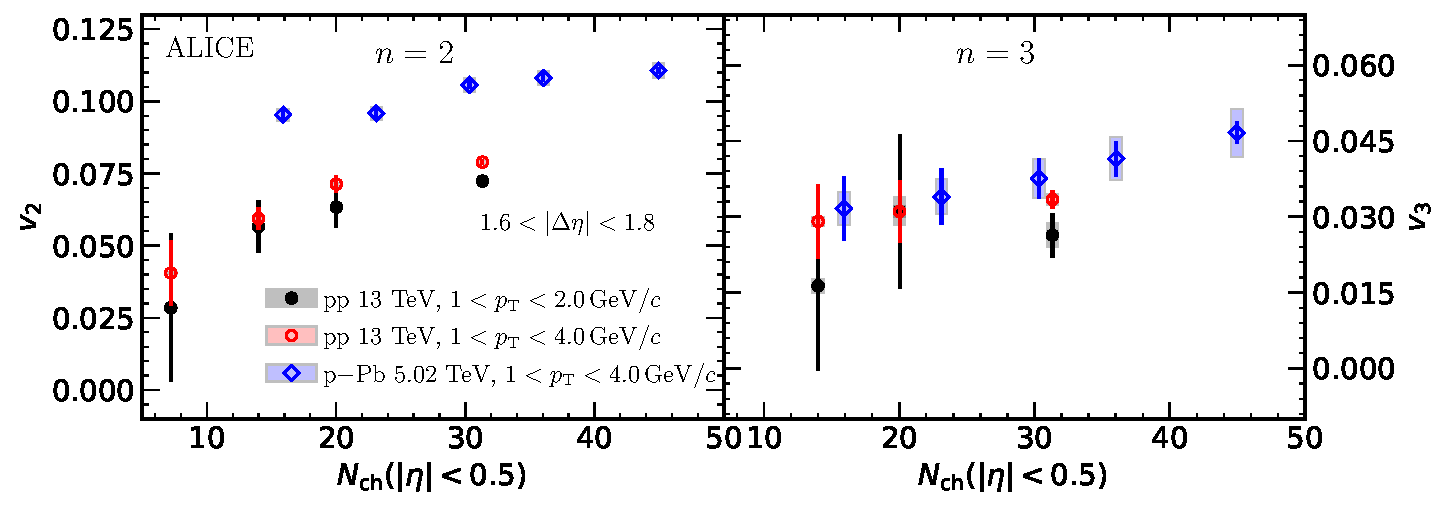
\includegraphics[width=1.0\textwidth]{figures/Fig6_v2Mult_allSystems_Data.pdf} 
	\caption{The $v_2$ magnitude for two different collision systems, pp and p-Pb, is presented as a function of multiplicity at mid-rapidity. For pp collisions, two different $p_\mathrm{T}$-intervals are shown, $1.0<p_\mathrm{T}<2.0$ GeV/c and $1.0<p_\mathrm{T}<4.0$ GeV/c.} 
	\label{fig:v2mult}
\end{figure}

In Fig.~\ref{fig:v2mult} the magnitude of $v_2$ as a function of multiplicity is presented for both pp at $\sqrt{s}=13$ and p--Pb collisions at $\sqrt{s_\mathrm{NN}}=5.02$ TeV. As in Fig.~\ref{fig:vn}, the large $\Delta\eta$ range is $1.6<|\Delta\eta|<1.8$ and the $v_2$ is measured in $1<p_{\mathrm{T}}<4\,\mathrm{GeV}/c$ for both collision systems. Additionally, the results in pp collisions at $\sqrt{s}=13$ with $1<p_{\mathrm{T}}<2$ GeV/$c$ are presented. Firstly, it is observed that the magnitude of $v_n$ increases with increasing multiplicity for both collision systems and $p_\mathrm{T}$-ranges. Secondly, $v_2$ in p--Pb is higher than in pp collisions in the measured multiplicity range. These two observations are compatible with previous results in Refs.~\cite{ATLAS:2015hzw,ATLAS:2016yzd, Khachatryan:2015lva}. The difference between the two collision systems is smaller for $v_3$, as shown on the right-hand side of Fig.~\ref{fig:v2mult}. Similar subtle multiplicity dependence is observed here as well, with larger values in higher multiplicity collisions.
%From~\cite{2016BSchenke} $v_n$ is expected to depend on the p--Pb collision geometry, however this dependence is not yet understood for pp collisions since by definition they  are only two colliding nucleons.
For the two different $p_\mathrm{T}$ intervals presented for the pp collisions, $v_2$ in $1.0<p_\mathrm{T}<4.0$ GeV/$c$ is larger than $v_2$ in $1.0<p_\mathrm{T}<2.0\,\mathrm{GeV}/c$ within the uncertainties. %and the ratio of the higher to low $p_\mathrm{T}$ results is shown in the bottom panel of Fig.~\ref{fig:v2mult}, showing about $1\%$ increase within the uncertainties.
This agrees with what is observed in Fig.~\ref{fig:vn}, where the $v_2$ magnitude has its largest value in $2.5<p_\mathrm{T}<3.0\,\mathrm{GeV}/c$. Within the uncertainty, no evidence of a $p_\mathrm{T}$-dependence is found for $v_3$.


\subsection{Event-scale dependence}
\begin{figure}[h!]
	\centering
	\hspace{-3em}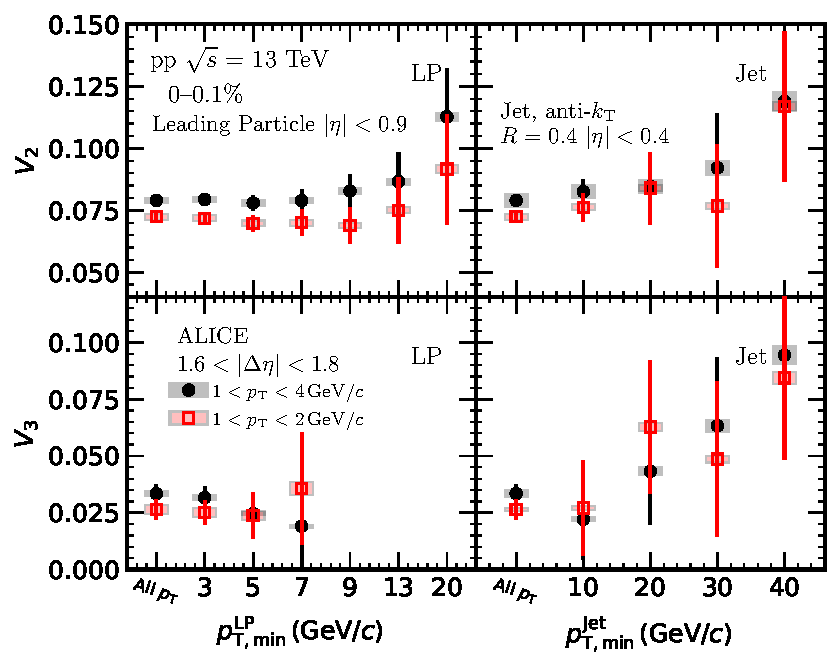
\includegraphics[width=0.8\textwidth]{figures/Fig4_vn_LP.pdf}
	\caption{The magnitude of $v_2$ (top) and $v_3$ (bottom) as a function of the $\it{p}^{\rm{LP}}_{\rm{T,min}}$ (left) and $\it{p}^{\rm{jet}}_{\rm{T,min}}$ (right) for the high multiplicity percentile of the 0--0.1\% in $\sqrt{s}=13$ pp collisions. The measured $p_{\mathrm{T}}$ intervals are $1<p_{\mathrm{T}}<2\,\mathrm{GeV}/c$ (in red) and $1<p_{\mathrm{T}}<4\,\mathrm{GeV}/c$ (in black). The statistical and systematic uncertainties are shown as vertical bars and boxes, respectively.}
	\label{fig:LPjet23}
\end{figure}    

Figure~\ref{fig:LPjet23} presents the extracted magnitude of $v_2$ and $v_3$ as functions of the minimum $p_\mathrm{T}$ of the leading particle $\it{p}^{\rm{LP}}_{\rm{T,min}}$ and that of the jet ($\it{p}^{\rm{jet}}_{\rm{T,min}}$) as used in the selection. 
Both event-scale results are obtained from the data in pp collisions at $\sqrt{s}= 13$ TeV for the 0--0.1\% multiplicity class and for two different $p_\mathrm{T}$-ranges, $1<p_{\mathrm{T}}<2\,\mathrm{GeV}/c$ in red and $1<p_{\mathrm{T}}<4\,\mathrm{GeV}/c$ in black. The leading particle is required to be within $|\eta|<0.9$ and the jets in this analysis are reconstructed using the anti-$k_\mathrm{T}$ algorithm with a distance parameter of $R=0.4$. To reduce the impact of the detector edge effects on the jet measurements, the jets are required to have a pseudorapidity $|\eta|<0.4$, following a similar approach as in Refs.~\cite{PhysRevD.65.092002, Aad:2011fc, Khachatryan:2014waa}. The $v_2$ and $v_3$ for both $p_\mathrm{T}$ ranges do not show any dependence on event-scale selection within the uncertainties. This finding is consistent with the results of the ridge yields~\cite{ALICE:2021nir} and $v_{2}$ measurements with a tagged $Z$ boson from the ATLAS collaboration~\cite{Aaboud:2019mcw}. These results suggest that the presence of a hard-scattering process does not significantly change the long-range correlation involving soft particles.
However, the measurements are only limited with low $\it{p}^{\rm{jet}}_{\rm{T}}$ and future measurements with multi-jet events at mid-rapidity with higher $Q^2$ reach can shed on the light on the expected impact parameter dependence~\cite{Sjostrand:1986ep,Frankfurt:2003td,Frankfurt:2010ea}.
%The $\pythiashoving$ model describes the ridge yields qualitatively while the $\epos$ model overestimating the ridge yield.

%While EPOS LHC (PYTHIA8 String Shoving) model shows a strong (weak) event-scale dependence and two models show different jet yields, it would be interesting to check how flow coefficients are related to the event-scale selections. However, up to date, it is not possible to extract flow coefficients with this LM-template method for these models because both models exhibit flow or ridge signals in LM events.

\subsection{Comparisons with models}
\label{sec:theory}

\begin{figure}[h!]
	\centering
	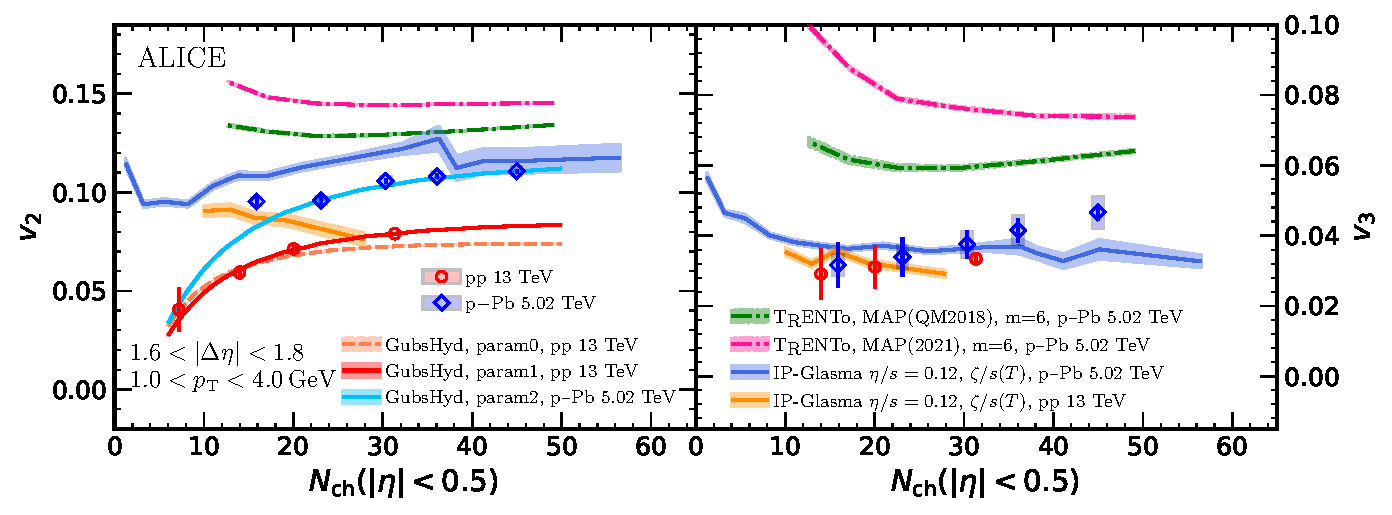
\includegraphics[width=1.0\textwidth]{figures/Fig6_v2Mult_allSystems_Hydro.pdf} 
	\caption{The $v_2$ (left) and $v_3$ (right) as a function of multiplicity at mid-rapidity is compared to the hydrodynamic calculations. The blue and red markers represent the p--Pb and pp collision data points, respectively. The hydrodynamic calculations are presented with colored lines and bands marking their statistical uncertainty.} 
	\label{fig:vnmult_model}
\end{figure}

In this section, the results are compared to various model calculations and the data to model comparison is shown in Fig.~\ref{fig:vnmult_model}.
The results from the data in p--Pb collisions are compared with hydrodynamic calculations using the parametrization from an improved global
Bayesian analysis of new sophisticated collective flow observables
 from two different beam energies in Pb--Pb collisions~\cite{Parkkila:2021yha}. This hydrodynamic model, {T\raisebox{-.5ex}{R}ENTo}+iEBE-VISHNU, consists of the {T\raisebox{-.5ex}{R}ENTo} model~\cite{Moreland:2014oya} for the initial condition, which is connected with a free streaming to a 2+1 dimensional causal hydrodynamic model VISH2+1~\cite{Shen:2014vra}. The evolution is continued after particlization with a hadronic cascade (UrQMD) model~\cite{Bass:1998ca,Bleicher:1999xi}. The initial conditions, $\eta/s(T)$, $\zeta/s(T)$ and other free parameters of the hybrid model are extracted in a global Bayesian analysis.
%incorporating constraints measured from a Pb--Pb collision system at $\sqrt{s_\mathrm{NN}}=5.02\,\mathrm{TeV}$.
A model calculation with the best-fit parameterization for the transport coefficients chosen by maximum a posteriori (MAP) for Pb--Pb collisions at $\sqrt{s_{\text{NN}}}=5.02$~TeV is performed as they are reported in Ref.~\cite{Parkkila:2021yha}. The parameterization for the initial conditions, which include a sub-nucleon structure with six constituent partons per nucleon, is taken from a model calibration with additional p--Pb data~\cite{Moreland:2018gsh}. All the kinematic cuts such as transverse momentum and pseudorapidity intervals are matched with the data reported in this article. The flow coefficients in the hydrodynamic calculation are extracted with the two-particle cumulant method, as the results are not affected by the away-side non-flow.

As shown in Fig.~\ref{fig:vnmult_model}, it is found that {T\raisebox{-.5ex}{R}ENTo}+iEBE-VISHNU overestimates both $v_2$ and $v_3$ by large margin. Whereas the data shows a multiplicity dependence with increasing values at larger multiplicities in the predicted multiplicity ranges, {T\raisebox{-.5ex}{R}ENTo}+iEBE-VISHNU predicts low values at higher multiplicities and higher values at low multiplicities, similarly as is found in large collision systems~\cite{Acharya:2020taj}. The large discrepancies in the prediction can be alleviated by inclusion of the newly measured p--Pb constraints in a future Bayesian parameter estimation as well as by the improvement of the initial condition model for the small collision systems.

The results are also compared with IP-Glasma+MUSIC+UrQMD hydrodynamic calculations~\cite{Schenke:2020mbo}. This model uses IP-Glasma initial conditions~\cite{Schenke:2012wb} including sub-nucleonic fluctuations with three hot-spots per nucleon. The hydrodynamic evolution is performed by MUSIC~\cite{Schenke:2010rr} and coupled with the UrQMD~\cite{Bass:1998ca,Bleicher:1999xi} hadronic interactions. 
% mean-pT All paramters are fixed to reproduce 200 GeV Au+Au collisions at RHIC and 
The model calculations are performed with a constant $\eta/s=0.12$ and a temperature dependent $\zeta/s(T)$~\cite{Rose:2020lfc}. 
This model describes well the multiplicity dependence of $v_2$ in p--Pb collisions and the magnitude at the highest multiplicity but overestimates the data for lower multiplicity classes. As for pp collisions, the calculations clearly miss both the observed magnitude except for $N_{ch}>25$ as well as the trend of the multiplicity dependence. The model shows that $v_2$ decreases with increasing multiplicity, while the experimental result shows an increase.
For $v_3$, the model accurately describes the magnitudes and multiplicity dependence across the measured multiplicity ranges. The magnitudes of $v_3$ are slightly smaller in pp collisions than in p--Pb collisions according to the calculations, which agrees with the data within the uncertainties.
%model missed important physics as the system becomes very small and the multiplicity very low, as is the case in p+p collisions, even though the initial T   does include initial state momentum anisotropies from the color glass condensate, as discussed in detail in [115]. arXiv:1908.06212 [nucl-th]. NEED to look further details.

Finally, the results are compared with the GubsHyd model which is a semi-analytical model based on the analytical Gubser solution that can be used to shed light on the possible sources of the observed discrepancy between the above mentioned models and the measurements in pp collisions~\cite{Taghavi:2019mqz}. In this model, instead of modeling the initial entropy density as typically done in T$_{\text{R}}$ENTo or IP-Glasma, the initial state fluctuation is modeled directly. It assumes that ellipticity $\epsilon_{2}$ and RMS radius $r_{\text{rms}}$ fluctuate independently with widths $\sigma_{\epsilon}$
 and $\sigma_{r}$, respectively. The multiplicity dependence of two-particle correlation functions $v_2\{2\}$ depends on $\sigma_{r}$ and  $\chi\sigma_{\epsilon}$ that can be obtained by comparing the model with data. Since no non-flow effect is considered in the calculation, $v_2\{2\}$ is comparable with flow measurements in the present study. The coefficient $\chi$ is fixed and encapsulates all the idealization of GubsHyd including the absence of the dissipation effects. The calculations for the two sets of parameters are compared
to the data in Fig.~\ref{fig:vnmult_model}. The “param0” parametrization is based on the prediction in Ref.~\cite{Taghavi:2019mqz} with $\chi \sigma_{\epsilon}$ = 0.097 and $\sigma_{r}$ = 0.4 fm. The other parametrization “param1” is with $\chi \sigma_{\epsilon}$ = 0.86 and $\sigma_{r}$ = 0.62 fm. Both calculations capture the multiplicity dependence of $v_2$ well and the calculations with larger $\sigma_{r}$ and smaller $\chi \sigma_{\epsilon}$ are preferred by the data.
 
\begin{comment}
\begin{figure}[h!]
	\centering
	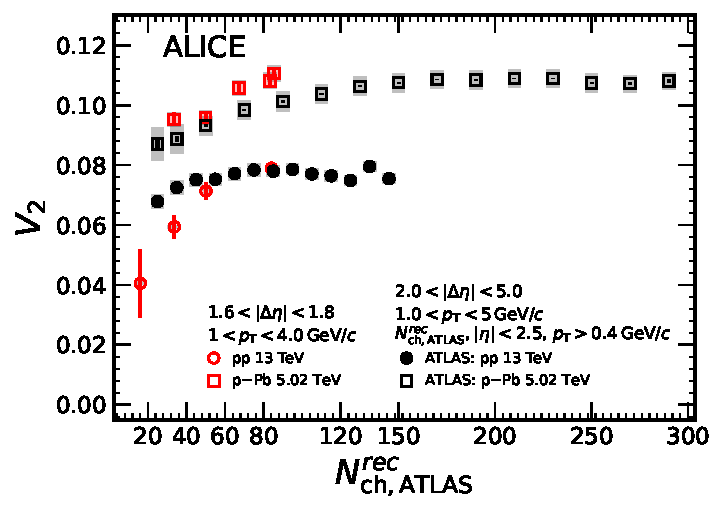
\includegraphics[width=0.45 \textwidth]{figures/Fig7_v2Mult_allSystemsATLAS.pdf} 
	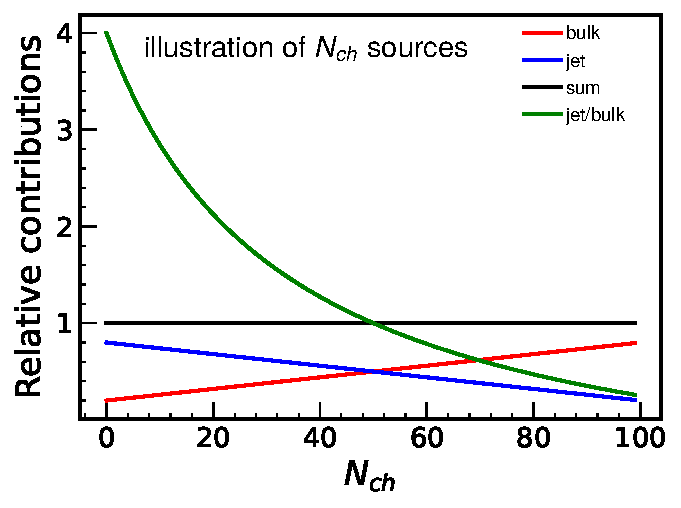
\includegraphics[width=0.425
	\textwidth]{figures/IllustrationNchSources.pdf} 
	\caption{Left: A comparison to ATLAS~\cite{Aaboud:2016yar} experiment of the $v_2$ magnitude for two different collision systems, pp and p-Pb, as a function of the ATLAS definition of multiplicity. Right: Illustration of sources of the measured multiplicity.} 
	\label{fig:v2multATLAS}
\end{figure}

The multiplicity dependent $v_2$ measurements in Fig.~\ref{fig:v2mult} are compared with the results by the ATLAS Collaboration~\cite{Aaboud:2016yar}. In case of the ATLAS measurement, the charged particle multiplicity was obtained by counting the number of reconstructed particles satisfying $\pt>0.4$~GeV/$c$ in $|\eta|<$~2.5. The ATLAS results have no efficiency correction (labeled as ${N^\mathrm{rec}_{\mathrm{ch},ATLAS}}$), therefore the result needs to take into account the efficiency reported in Ref.~\cite{ATLAS:2016yzd} to be compared to our measurements, which are 1.29$\pm$0.05 and 1.18$\pm$0.05 in p--Pb and pp collisions, respectively. In our analysis, the reference multiplicity is measured by integrating the $\dndeta$ in $|\eta|<0.5$ for each multiplicity percentile measured by the V0M and V0A in pp and p--Pb collisions, respectively. The ATLAS reference multiplicity definition is $|\eta|<2.5$ with $p_\mathrm{T}>0.4$ GeV/$c$ for both collision systems. 
The measured ALICE multiplicity percentiles are converted to the ATLAS definition by integrating the $\dndeta$ results for $\pt>0.4$~GeV/$c$ in their respective $\eta$-ranges using EPOS LHC simulation. 
The difference in multiplicity between the respective $\eta$-ranges, assuming that the $\eta$-distribution is flat. This is reduced to a factor of $\sim$three when requiring $p_\mathrm{T}>0.4$ GeV/c, i.e., a noticeable effect.
The EPOS LHC does not match with the measurements completely in $|\eta|<$~0.8 and it is scaled to the measurements before the integration. Based on the studies in Ref.~\cite{ALICE:Nchpt}, the measured ALICE $\dndeta$ within $|\eta|<$~0.8 with various $\pt$ cut-offs is compatible to the measurements by ATLAS and CMS as well as EPOS LHC simulations. Finally, the comparison of our results to ATLAS is shown in Fig.~\ref{fig:v2multATLAS} as a function of ${N^\mathrm{rec}_{\mathrm{ch},ATLAS}}$.  
Our results in p--Pb collisions agree with those of ATLAS in lower multiplicity and are slightly larger for our highest multiplicity interval. In case of pp collisions, our results agree better with the results by ATLAS for the highest two multiplicity intervals but are smaller in ${N^\mathrm{rec}_{\mathrm{ch},ATLAS}}<40$. 
\end{comment}

In summary, the measured $v_{2}$ from both experiments decreases with decreasing multiplicity for both pp and p--Pb collisions, which is also predicted in the GubsHyd model calculations~\cite{Taghavi:2019mqz} and in Ref.~\cite{Weller:2017tsr}. Interestingly, the opposite situation can be seen in pp collisions, where $v_2$ decreases with increasing multiplicity according to IP-Glasma+MUSIC+UrQMD hydrodynamic calculations~\cite{Schenke:2020mbo}. 
Approaching a lower bound for the size of a hydrodynamized
system as predicted in Ref.~\cite{Taghavi:2019mqz}, 
the decreasing trend of $v_2$ by lowering the multiplicity changes and raise again after a minimum value. However, this change in multiplicity dependence of $v_2$ at low multiplicities is still challenging to test with the current experimental uncertainties. In case of $v_3$, only IP-Glasma+MUSIC+UrQMD hydrodynamic calculations~\cite{Schenke:2020mbo} accurately describes the magnitudes and multiplicity dependence across the measured multiplicity ranges where the magnitudes of $v_3$ are slightly smaller in pp collisions than in p--Pb collisions according to the calculations. The discrepancies in the prediction of the data can be further studied by including these measurements in a future Bayesian parameter estimation, as well as by improving the initial condition model for the small collision systems.

%One has to note that the different sources of the multiplicity between the models and data can be considered where the measured $v_n$ might be averaged over different events. The relative jet and bulk particle's yields vary with the measured $N_{ch}$. This results in lower $v_2$ values on average in low multiplicity events. While the data are compared to hydrodynamic model calculations which contain only bulk particles, the difference in $N_{ch}$ should be taken into account carefully and this work needs further investigations and needs to be left for future work because it requires adequate treatments of jet and bulk particle productions in both experiment and theory.
